% !TeX spellcheck = en_US
\section{Introduction}
\subsection{Computer}
\begin{wrapfigure}{r}{5.5cm}
	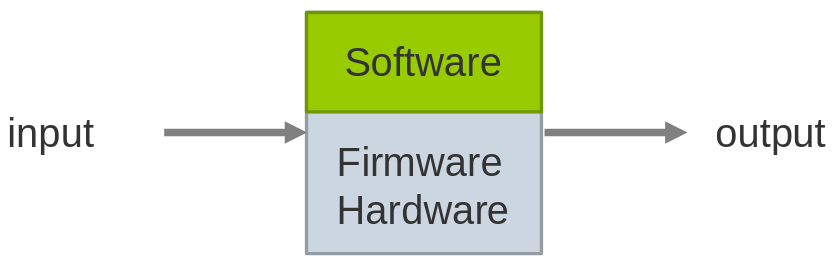
\includegraphics[scale=0.17]{components}
\end{wrapfigure}
A computer is made of three components:
\begin{itemize}
	\item \textbf{Hardware}: mechanical and electronic components
	\item \textbf{Software}: programs running on it
	\item \textbf{Firmware}: micro-programs stored in ROM
\end{itemize}

\begin{note}
	Logical equivalence between HW and SW.
\end{note}

\subsubsection{Micro-Computer}
A micro-computer classical architecture is composed of different \textbf{modules}, each one dedicated to a feature (and to a corresponding physical part). They're all connected through a \textbf{bus}.
\begin{center}
	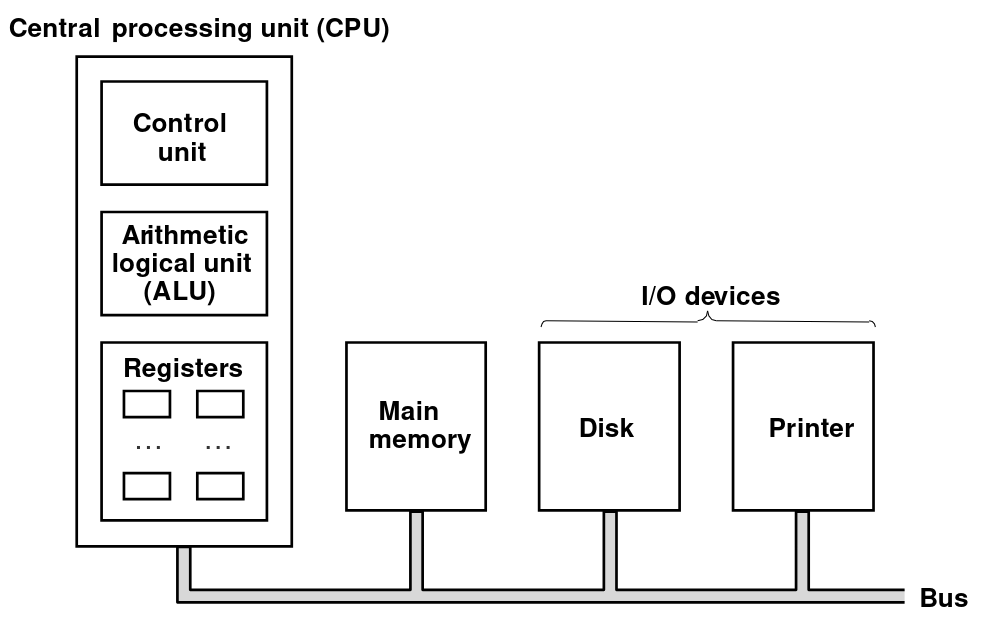
\includegraphics[scale=0.3]{microcomp}
\end{center}

\subsection{Architecture}
\subsubsection{Von Neumann}
\begin{wrapfigure}{r}{3.5cm}
	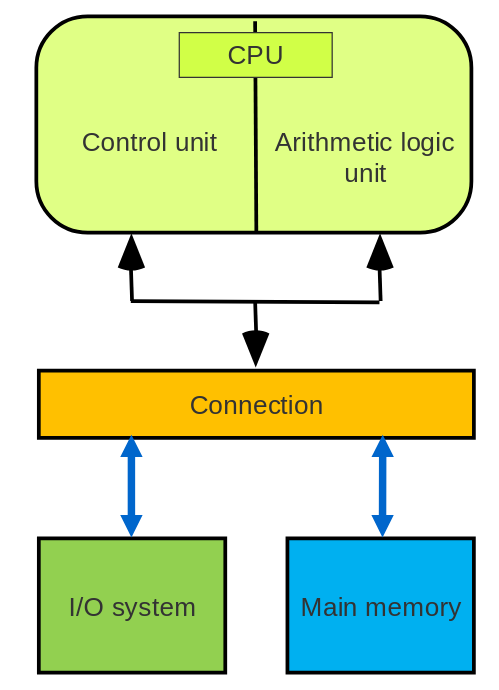
\includegraphics[width=3.5cm]{vonneumann}
\end{wrapfigure}
This architecture is one of the most wide spread. It has the following components:
\begin{itemize}
	\item \textbf{Central Processing Unit}: controls the flow and the execution of all instructions. Consists of:
	\begin{itemize}
		\item \textbf{Control Unit}: interprets the instructions and generates the control commands for other components
		\item \textbf{Arithmetic Logical Unit}: executes the instructions, if needed with I/O and memory modules
	\end{itemize}
	\item \textbf{Memory}: storage of \textbf{data} and \textbf{programs} as sequences of bits. It consists of memory cells with a fixed length, each one accessed individually with an address.
	\begin{center}
		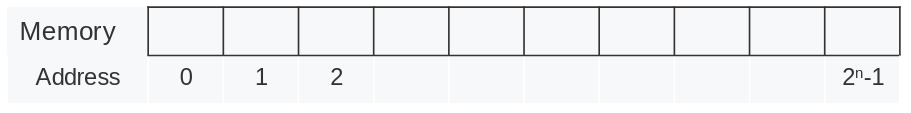
\includegraphics[scale=0.25]{memory}
	\end{center}
	\item \textbf{Input/Output} units: interface to the outside world that inputs and outputs the data
	\item \textbf{Interconnection}
	\begin{observation}[Von Neumann Bottleneck]
		Since there is no difference in memory between instructions and data and the CPU is way faster than the bus and the memory, the main interconnection is the central bottleneck.
	\end{observation}
\end{itemize}

\paragraph{IBM PC}
The IBM PC is a modified von Neumann architecture and was introduced by IBM fall 1981. The interconnection structure was realized by several busses.
\begin{center}
	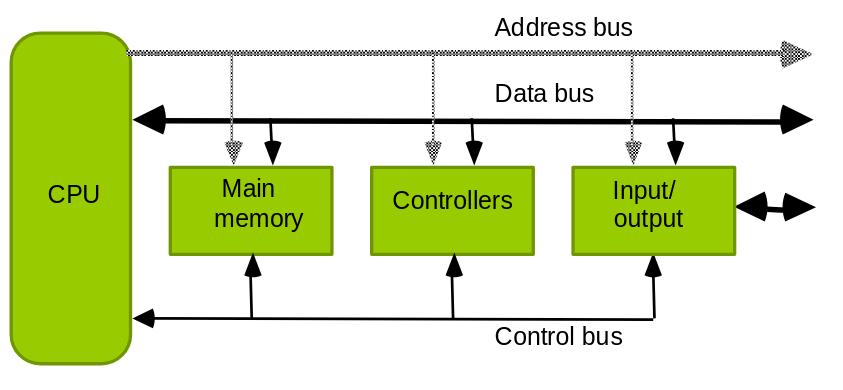
\includegraphics[scale=0.3]{ibmpc}
\end{center}

\paragraph{Principle of operation}
This architecture follows the \textbf{Single Instruction Single Data} (SISD): at any time the CPU executes only a single instruction that can only manipulate a single operand.\\\\
There are \textbf{no memory protection} mechanisms, meaning that programs can destroy each other and access arbitrary data. Memory is \textbf{unstructured} and is addressed linearly. Interpretation of memory content depends on the context of the current program only.\\\\
Instruction processing follows a two phase principle:
\begin{itemize}
	\item \textbf{Interpretation}: the content of a memory cell is fetched based on a program counter. This
	content is then interpreted as an instruction.	
	\item \textbf{Execution}: the content of a memory cell is fetched based on the address contained in the
	instruction. This content is then interpreted as data.
\end{itemize}
\begin{note}
	The instruction flow follows a strict \textbf{sequential} order.	
\end{note}

\paragraph{Pros and cons}
The \textcolor{green}{\textbf{advantages}} of this architecture:
\begin{itemize}
	\item Principle of minimal HW requirement
	\item Principle of minimal memory requirement
\end{itemize}
The \textcolor{red}{\textbf{disadvantages}}:
\begin{itemize}
	\item Von Neumann bottleneck, also influencing programming approaches to deal with that
	\item Low structuring of data
	\item The instruction determines the operand type
\end{itemize}

\subsubsection{Harvard}
The main idea in this architecture is that there is a separation between data and program memory. Typically a processor uses this internally and then externally has a Von Neumann.
\begin{center}
	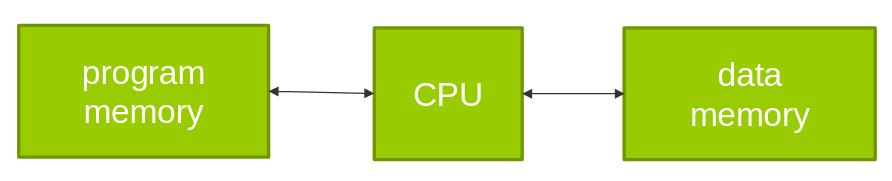
\includegraphics[scale=0.3]{harvard}
\end{center}

\subsection{Performance}
\begin{definition}[Moore's Law]
	The number of transistors in an integrated circuit doubles about every two years. 
\end{definition}

\begin{observation}[Overclocking]
	Given a certain processor with a clock speed, we can tune it up. The main consequence is that the energy used increases drastically, leading to higher and higher temperatures.
\end{observation}

We need to assess the performance of a computer for different reasons: selecting a new one, tuning it o designing it. There are different methods to do so:
\begin{itemize}
	\item Evaluation of \textbf{hardware parameters}, such as
	\begin{itemize}
		\item Hypothetical maximum performance
		\item \textbf{MIPS} o \textbf{MOPS}: millions of instructions/operations per second
		\item \textbf{MFLOPS}: millions of floating point operations per second
		\item \textbf{MLIPS}: millions of logical interferences per second
	\end{itemize}
	\item \textbf{Run-time measurements} of existing programs through \textbf{benchmarks} that do different tasks (e.g. number crunching)
	\item \textbf{Monitoring} real cases of users through HW and SW monitoring
	\item Model \textbf{theoretic} approach with analytical methods or SW simulations
\end{itemize}

\paragraph{Benchmarks}
Here some example of benchmarks:
\begin{itemize}
	\item \textbf{Sieve of Erathostenes}: uses the Ackermann function
	\item \textbf{Whetstone}: from 1970, uses FORTRAN with a lot of floating point arithmetic
	\item \textbf{Dhrystone}: from the begin of 1980s, focused on integers
	\item \textbf{Savage-Benchmark}: with mathematical standard functions
	\item \textbf{Basic Linear Algebra Subprograms} (BLAS), which is the core of the Linear Algebra Package
	\item \textbf{Lawrence Livermore Loops} for vectorizing compilers
	\item \textbf{SPEC}: Standard Performance Evaluation Corporation is a non profit organization created in 1989 that involves a lot of chip vendors. They focus on calculation speed and throughput.
\end{itemize}

\subsection{Instruction Set Architecture}
This type of architecture comprises the description of \textbf{attributes} and \textbf{functions} of a system from a machine language programmer's point of view. It enables the use of programs independent on the actual implementation. It defines:
\begin{itemize}
	\item Instruction set
	\item Instruction formats
	\item Addressing modes
	\item Interrupt handling
	\item Logical address space
	\item Register and memory model accessible by the programmer
\end{itemize}
\begin{note}
	It does not describe internal operations, components and implementation.
\end{note}

\subsection{Micro Architecture}
This type of architecture comprises the description of \textbf{hardware structure}, \textbf{data paths}, and \textbf{internal logic} of a specific realization of a processor. It defines:
\begin{itemize}
	\item Number and stages of pipelines
	\item Usage of super scalar technology
	\item Number of ALUs
	\item Organization of cache memory
\end{itemize}

\begin{definition}[Binary compatibility]
	All microprocessors following the same processor architecture specification are called \textbf{binary compatibles}.
\end{definition}

\subsection{Classification}
To classify different architectures we use the type of supported \textbf{parallelism}.\\
A parallel program can be seen as a partially ordered set of instructions, where the order is given by the dependencies among them. Independent instructions can be executed in parallel.\\
We have five levels of parallelism:
\begin{enumerate}
	\item \textbf{Program}
	\item \textbf{Process} or \textbf{task}: it involves heavy weighted processes or coarse-grained tasks
	\item \textbf{Block}: it involves threads or light-weighted processes
	\item \textbf{Instruction}: about the basic instructions of the chosen language or instruction set
	\item \textbf{Sub-Operation}: basic instructions of a language or instruction set can be divided into sub-operations/micro operations by a compiler/the processor
\end{enumerate}

\paragraph{Granularity}
The granularity depends on the relation of computation effort over communication or synchronization effort. Typically we have:
\begin{itemize}
	\item \textbf{Large} grained: program, process, and thread level 
	\item \textbf{Fine} grained: instruction and sub-operation
\end{itemize}
\begin{note}
	Sometimes, the block or thread level is considered as \textbf{medium} grained.	
\end{note}

\subsection{6-Level model}
\begin{center}
	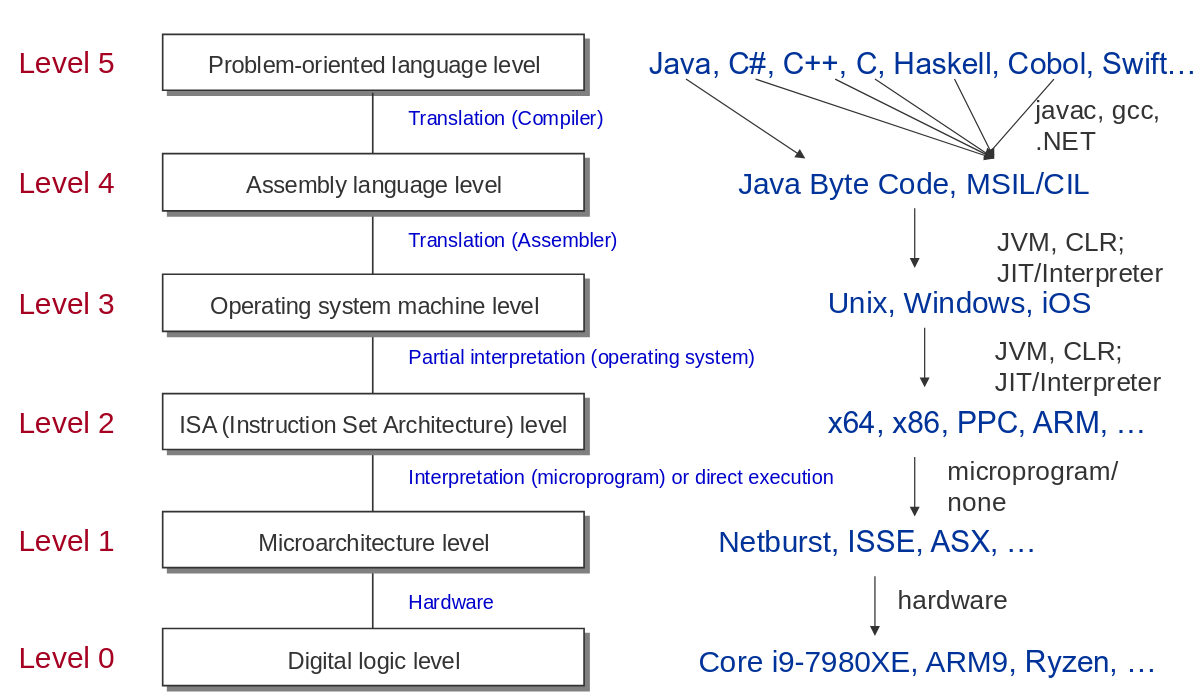
\includegraphics[scale=0.3]{6level}
\end{center}